\documentclass[10pt,a4paper]{report}
\usepackage[utf8]{inputenc}
\usepackage[spanish]{babel}
\usepackage{amsmath}
\usepackage{amsfonts}
\usepackage{amssymb}
\usepackage{lmodern}
\usepackage[left=2cm,right=2cm,top=2cm,bottom=2cm]{geometry}
\usepackage{makeidx}
\usepackage{graphicx}
\usepackage{lmodern}


\title{Resumen Paradigmas de la Programación\\~\\Licenciatura en Ciencias de la 
Computación\\FaMAF-UNC}
\author{Agustin Curto     agucurto95@gmail.com}
\date{2016}

\begin{document}
\tableofcontents

\chapter{Qué es y qué puede hacer un lenguaje de programación}

    Un lenguaje de programación es un lenguaje formal diseñado para realizar procesos que pueden ser llevados a cabo 
    por máquinas como las computadoras. Pueden usarse para crear programas que controlen el comportamiento físico y 
    lógico de una máquina o para expresar algoritmos con precisión.

    \section{Sintáxis y Semántica}

        \par Los lenguajes son sistemas que se sirven de una forma para comunicar un significado. Lo que tiene que ver 
            con la forma recibe el nombre de \textbf{sintaxis} y lo que tiene que ver con el significado recibe el 
            nombre de \textbf{semántica}.

        \par En los lenguajes de programación, que son lenguajes artificiales creados por hombres (lenguajes normales),
            la forma son los programas y el significado es lo que los prográmas hacen, usualmente, en una computadora.
            En la definición de arriba, se ha descrito lo que los programas como “controlar el comportamiento físico y 
            lógico de una máquina”.

        \par Un lenguaje de programación se describe con su sintáxis (qué es lo que se puede escribir legalmente en ese
            lenguaje) y su semántica (qué efectos tiene en la máquina lo que se escribe en ese lenguaje).

        \par La implementación de un lenguaje de programación debe transformar la sintáxis de un programa en 
            instrucciones de máquina que se pueden ejecutar para que suceda la secuencia de acciones que se pretendía. 
            El compilador hace esa traducción, un intérprete puede combinar traducción y ejecución.

    \section{ Sintáxis a traves de gramáticas}

    \par Vamos a estar usando gramáticas independientes de contexto, más específicamente EBNF, que es el estándar de   
        facto para estas gramáticas; aunque algunas propiedades de los lenguajes de programación escapan a su 
        expresividad.

    \par Un gramática es un método para definir conjuntos infinitos de expresiones y procesar expresiones. Consisten 
        de: 

        \begin{itemize}
            \item símbolo inicial
            \item no terminales
            \item terminales
            \item producciones
        \end{itemize}

    \par Los no terminales son la forma adecuada de describir la composicionalidad de las expresiones, no pueden formar
        parte de una expresión, siempre se tienen que substituir por terminales.

\chapter{Cómo funcionan los lenguajes de programación}

    \section{Compilador}

        \par El compilador es un programa que lee un programa escrito en un lenguaje origen y lo traduce a un programa 
            equivalente en un lenguaje destino, normalmente el lenguaje origen es de alto nivel y el destino es de 
            bajo nivel. El mismo posee dos componentes:

        \begin{itemize}
            \item Entender el programa (asegurarse de que es correcto)
            \item Reescribir el programa
        \end{itemize}

        \subsection{Fases de un compilador}

            \begin{enumerate}
                \item \underline{Análisis léxico:} se divide un programa (secuencia de caracteres) en palabras
                    (tokens).
                
                \item \underline{Análisis sintáctico:} comprueba si la secuencia de tokens conforma a la especificación
                    gramatical del lenguaje y genera el árbol sintáctico. La especificación gramatical suele 
                    representarse con una gramática independiente de contexto, que también le da forma al árbol 
                    sintáctico.
                
                \item \underline{Análisis semántico:} El compilador trata de ver si un un programa tiene sentido 
                    analizando su árbol sintáctico. Un programa sin errores gramaticales no siempre es correcto, puede 
                    haber problemas de tipo:

                    \begin{equation}
                        pos =  init + rate * 60
                    \end{equation}
                
                    \par Qué pasa si pos es una clase y init y rate son enteros. El parser no puede encontrar este 
                        tipo de errores, el análisis semántico encuentra este tipo de error.

                    \par El compilador hace comprobaciones semánticas estáticas (static semantic checks): 
                        
                        \begin{itemize}
                            \item comprobación de tipos
                            \item declaración de variables antes de su uso
                            \item se usan los identificadores en contextos adecuados 
                            \item comprobar argumentos
                        \end{itemize}

                    \par Si hay un fallo en compilación, se genera un error en tiempo de ejecución (dynamic semantic 
                        check) se comprueba:

                        \begin{itemize}
                            \item que los valores de los arreglos estén dentro de los límites
                            \item errores aritméticos (división por 0)
                            \item no se desreferencian los punteros si no apuntan a un objeto válido 
                            \item se usan variables sin inicialización
                            \item si hay un fallo en ejecución, se levanta una excepción
                        \end{itemize}
                    
                        \subsubsection{Tipado fuerte}
                        
                        \par Un lenguaje tiene tipado fuerte si siempre se detectan los errores de tipo:

                        \begin{itemize}

                            \item En tiempo de compilación o de ejecución
                            \item Tipado fuerte: Ada, Java, ML, Haskell
                            \item Tipado débil: Fortran, Pascal, C/C++, Lisp 
                            \item Duck typing: Python
                        
                            \par El tipado fuerte hace que el lenguaje sea más seguro y fácil de usar sin errores, pero 
                                potencialmente más lento por las comprobaciones dinámicas. En algunos lenguajes algunos 
                                errores de tipo se detectan tarde, lo que los hace poco fiables (Basic, Lisp, 
                                Prolog, lenguajes de scripting).
                        \end{itemize}
                    
                \item \underline{Generación y optimización de código intermedio:} El código intermedio está cerca de 
                    la máquina pero sigue siendo fácil de manipular, para poder implementar optimizaciones. Por ejemplo:
                
                    \begin{equation}
                        temp1 = 60
                    \end{equation}
                    \begin{equation}
                        temp2 = id3 + temp1
                    \end{equation}
                    \begin{equation}
                        temp3 = id2 + temp2
                    \end{equation}
                    \begin{equation}
                        id1 = temp3 
                    \end{equation}

                    \par Se puede optimizar (independientemente de máquina):
                    
                    \begin{equation}
                        temp1 = id3 * 60.0
                    \end{equation}
                    \begin{equation}
                        id1 = id2 + temp1 
                    \end{equation}

                \item \underline{Generación y optimización de código destino:} De la forma independiente de máquina se 
                    genera ensamblador:
                    \begin{equation}
                     MOVF id3, R2
                     \end{equation}
                     \begin{equation}
                     MULF 60.0, R2
                     \end{equation}
                     \begin{equation}
                     MOVF id2, R1
                     \end{equation}
                     \begin{equation}
                     ADDF R2, R1
                     \end{equation}
                     \begin{equation}
                     MOVF R1, id1
                     \end{equation}
                     
                     \par Este código específico de máquina se optimiza para explotar características de hardware 
                        específicas.
            
            \end{enumerate}


    \section{Paradigma Imperativo}

        \par Un paradigma de programacón es una configuracón frecuente de características de lenguajes de programacón. El 
            paradigma imperativo es el más antiguo y el que estuvo siempre más pegado a la máquina. Tradicionalmente se ha 
            opuesto al paradigma funcional, pero la mayor parte de lenguajes integran ideas de ambos paradigmas.

        \subsection{Conceptos fundamentales}

            \begin{itemize}
                \item Operación básica: \textbf{asignación}. La asignación tiene efectos secundarios ya que cambia el 
                    estado de la máquina.
                \item Sentencias de \textbf{control} de flujo: condicionales y sin condición (GO TO), ramas, ciclos.
                \item Bloques, para obtener \textbf{referencias locales}
                \item \textbf{Parametrización}
            \end{itemize}

        \subsection{Elementos básicos}
            
            \begin{enumerate}
                \item Definiciones de \textbf{tipos}
                \item Declaraciones de \textbf{variables} (normalmente tipadas)     
                \item Expresiones y sentencias de \textbf{asignación}
                \item Sentencias de \textbf{control de flujo} (normalmente estructuradas)
                \item \textbf{Alcance léxico} y bloques, para poder tener variables con referencias locales
                \item Declaraciones y definiciones de \textbf{procedimientos} y 
                \textbf{funciones} (bloques parametrizados)
            \end{enumerate}
                
        \subsection{Declaraciónes de variables}

            \par Las declaraciones tipadas restringen los posibles valores de una variable en la ejecución del programa:
                
                \begin{itemize}
                    \item Jerarquía de tipos built-in o personalizada
                    \item inicialización
            \end{itemize}
                
            \par Uso de memoria: cuánto espacio de memoria reservar para cada tipo de variable.
              
        \subsection{Ubicación y valores de variables}
            \par Al declarar una variable la estamos ligando a una \textbf{ubicación en memoria}, de forma que el nombre 
                de la 
                variable es el identificador de la ubicación en memoria. La ubicación puede ser global, en la pila o en el 
                heap.
            \begin{itemize}
                \item l-valor: ubicación en memoria (dirección de memoria)
                \item r-valor: valor que se guarda en la ubicación de memoria 
                identificada por el l-valor
            \end{itemize}
                
            \par La asignación: A (objetivo) = B (expresión), es una actualización destructiva, ya que reescribe la ubicación 
                de memoria identificada por A con el valor de la expresión B.

        \subsection{Semántica de copia vs. Semántica de referencia}
                \begin{itemize}
                    \item Semántica de copia: la expresión se evalúa a un valor, que se copia al objetivo (lenguajes 
                        imperativos).
                    \item Semántica de referencia: la expresión se evalúa a un objeto, cuyo puntero se copia al objetivo
                        (lenguajes orientados a objetos).
                \end{itemize}

        \subsection{Variables y asignación}
            \par En la parte derecha de una asignación está el r-valor de la variable, en la parte izquierda está su l-valor. 
                Una expresión que no tenga un l-valor no puede aparecer en la parte izquierda de una asignación. El r-valor de 
                un puntero es el l-valor de otra variable (el valor de un puntero es una dirección).
                
                \begin{itemize}
                    \item las constantes sólo tienen r-valor
                    \item las funciones sólo tienen l-valor
                \end{itemize}

            \subsubsection{L-valor y R-valor en C}
                \begin{itemize}
                    \item \&x devuelve el l-valor de x 
                    \item *p devuelve el r-valor de p. Si p es un puntero, esto es el l-valor de otra variable
                \end{itemize}

        \subsection{Control de flujo estructurado}

            \par Se piensa como secuencial, las instrucciones se ejecutan en el orden en el que están escritas, en algunos
                casos soporta ejecución concurrente. \par Un programa es estructurado si el flujo de control es evidente en la 
                estructura sintáctica del texto del programa. Esto es     útil para poder razonar intuitivamente leyendo el 
                texto del programa, ya que se crean construcciones del lenguaje para patrones comunes de control: iteración, 
                selección, procedimientos, funciones, etc.

            \subsubsection{Estilo moderno}
                \par Construcciones estándar que estructuran los saltos: 
            
                \begin{itemize}
                    \item if ... then ... else ... end 
                    \item while ... do ... end
                    \item for ...{...}
                    \item case ...
                \end{itemize}
                
            \par Se agrupa el código en bloques lógicos, se evitan saltos explícitos (excepto retorno de función), no se puede 
                saltar al medio de un bloque o función.


\chapter{Estructura en bloques}

\section{Estructura de bloque}
\subsubsection{Manejo de memoria}
        \begin{itemize}
            \item Al stack tiene los datos sobre entrada y salida de bloques
            \item El heap tiene datos de diferente lifetime
            \item El puntero de entorno (environment) apunta a la posición 
            actual en el stack
            \item Al entrar a un bloque: se añade un nuevo activation record al 
            stack
            \item Al salir de un bloque: se elimina el activation record más 
            reciente del stack
        \end{itemize}
        
\subsection{Alcance y lifetime}
\begin{itemize}
\item Alcance: región del texto del programa donde una declaración es 
visible.
\item Lifetime: período de tiempo en que una ubicación de memoria es asignada a un programa.
\end{itemize}

\section{Activation records}

\par Para describir la semántica de los lenguajes de programación, más 
específicamente lenguajes estructurados por bloques, usamos una 
semántica operacional, es decir, describimos los efectos de las diferentes 
expresiones del lenguaje sobre una máquina. Para eso usamos un modelo 
simplificado de la computadora, el que se ve en la figura.

\begin{center} 
    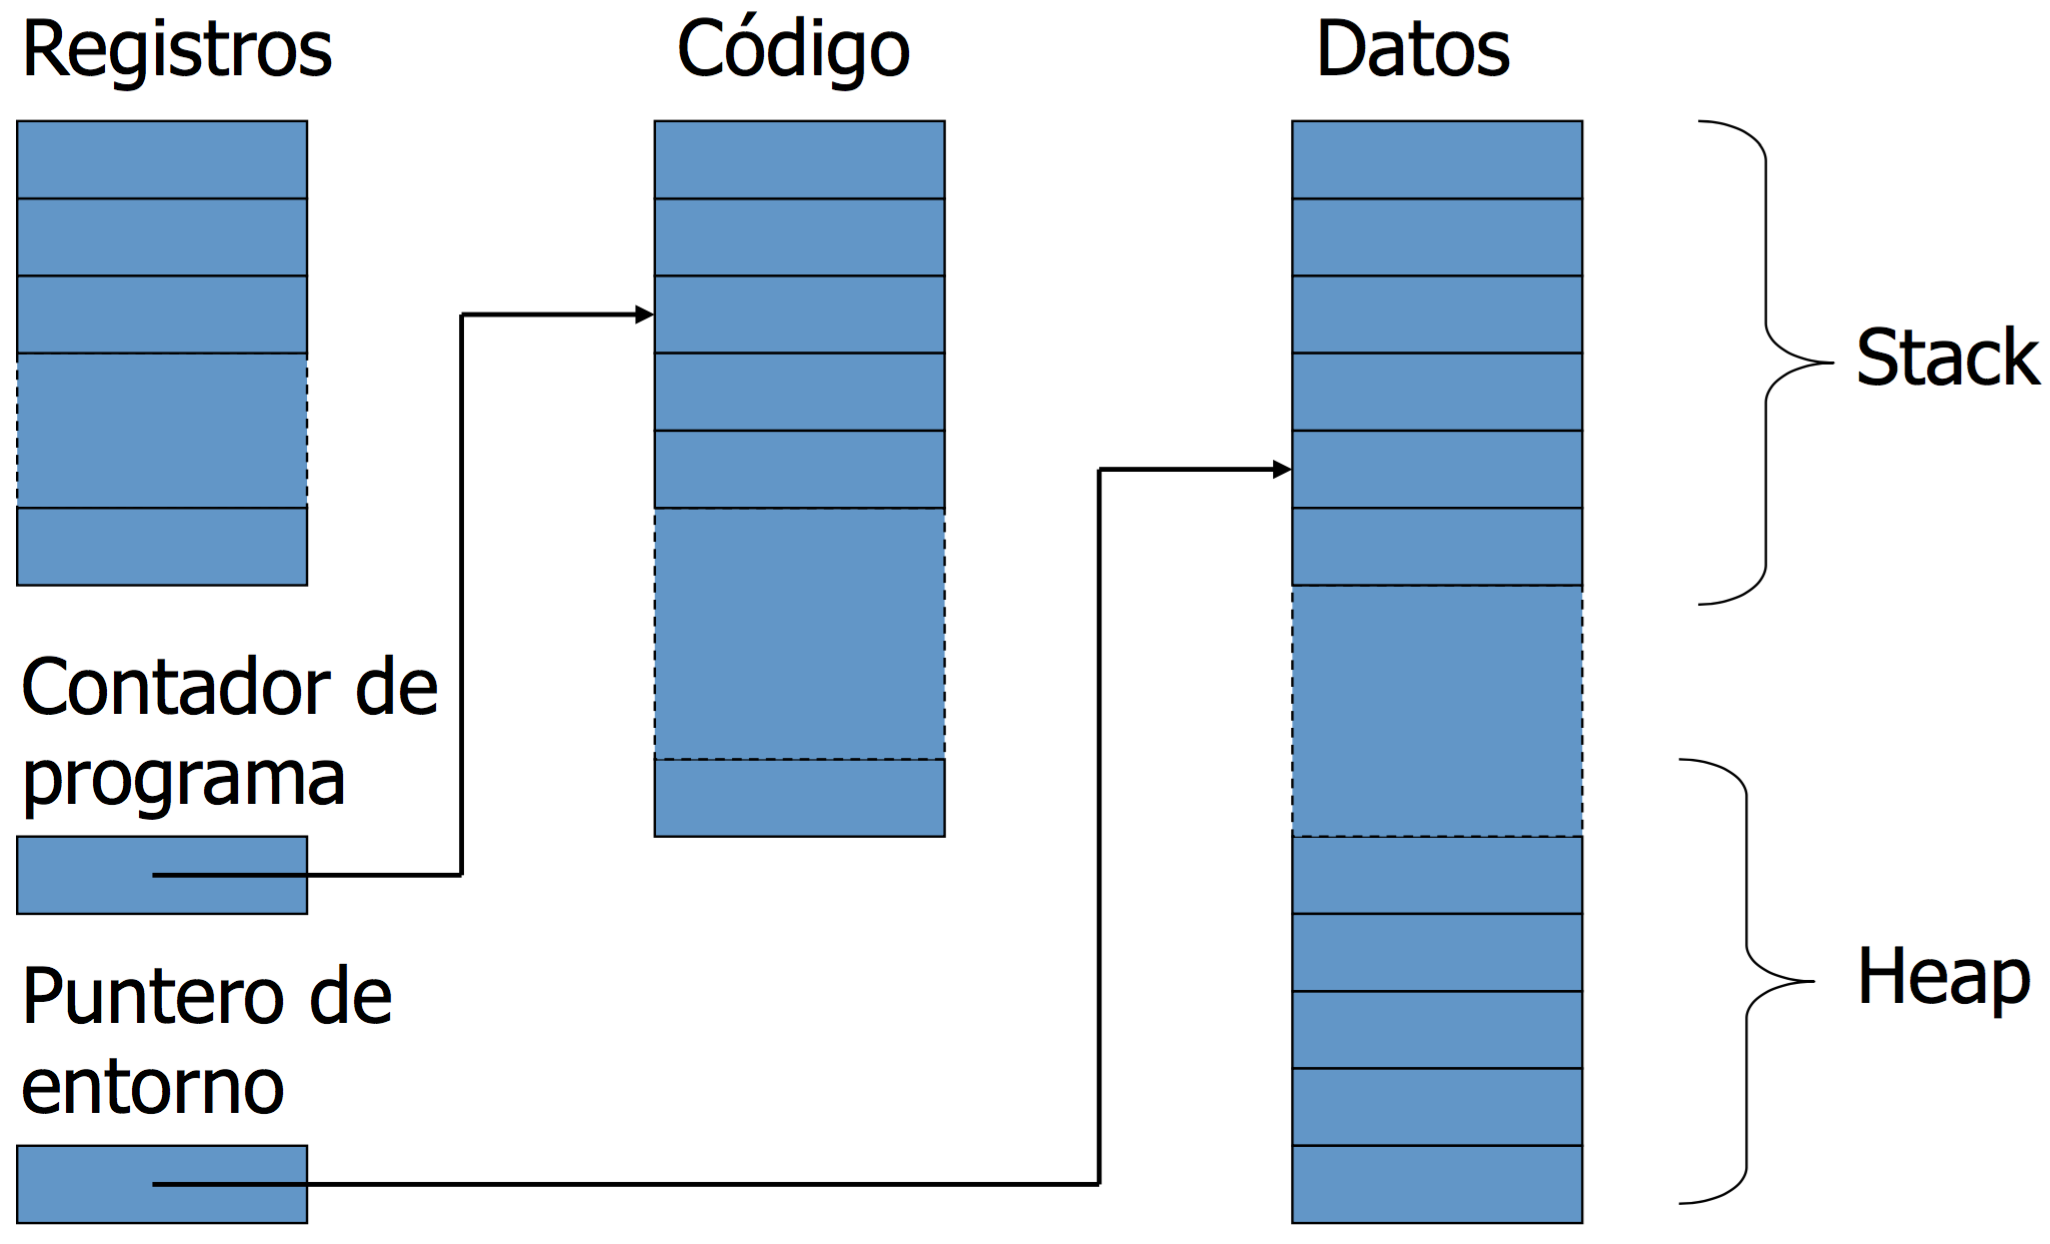
\includegraphics[width=12cm, height=6cm]{arecord.png}
\end{center}

\par Vemos que este modelo de máquina separa la memoria en la que se 
guarda el código (\textbf{stack}), de la memoria en la que se guardan los 
datos (\textbf{heap}). Usamos dos variables para saber a qué parte de la 
memoria necesitamos acceder en cada momento de la ejecución del 
programa: el \textbf{contador de programa}, que es una dirección en la 
parte de la memoria donde se guarda el código, en concreto, la dirección 
donde se encuentra la instrucción de programa que se está ejecuntando 
actualmente y y el \textbf{puntero de entorno}, el cual nos sirve para 
saber cuáles son los valores que se asignan a las variables que se están 
usando en una parte determinada del código. 

\par Cuando el programa entra en un nuevo bloque, el stack se encarga de agregar una estructura de datos que se llama \textbf{\textit{activation record}}, que contiene el espacio para las variables locales declaradas en el bloque, normalmente, por la parte de arriba de la pila. Entonces, el puntero de entorno apunta al nuevo activation record.

\par Cuando el programa sale del bloque, se retira el activation record de la pila y el puntero de entorno se restablece a su ubicación anterior, es decir, al puntero de entorno correspondiente a la función que llamaba a la función que ha sido desapilada. El activation record que se apila más recientemente es el primero en ser desapilado, a esto se le llama disciplina de pila.

\par Ademas el activation record posee espacio para guardar resultados intermedios, en el caso de que sea necesario. Podemos observar, en la figura siguiente, que hay dos direcciones de memoria donde se guardan datos importantes: el control link, contiene el que será el puntero de entorno cuando se desapile el activation record actual y la dirección de memoria distinguida es la llamada dirección de retorno, que es donde se va a guardar el resultado de la ejecución de la función, si es que lo hay.

\begin{center} 
        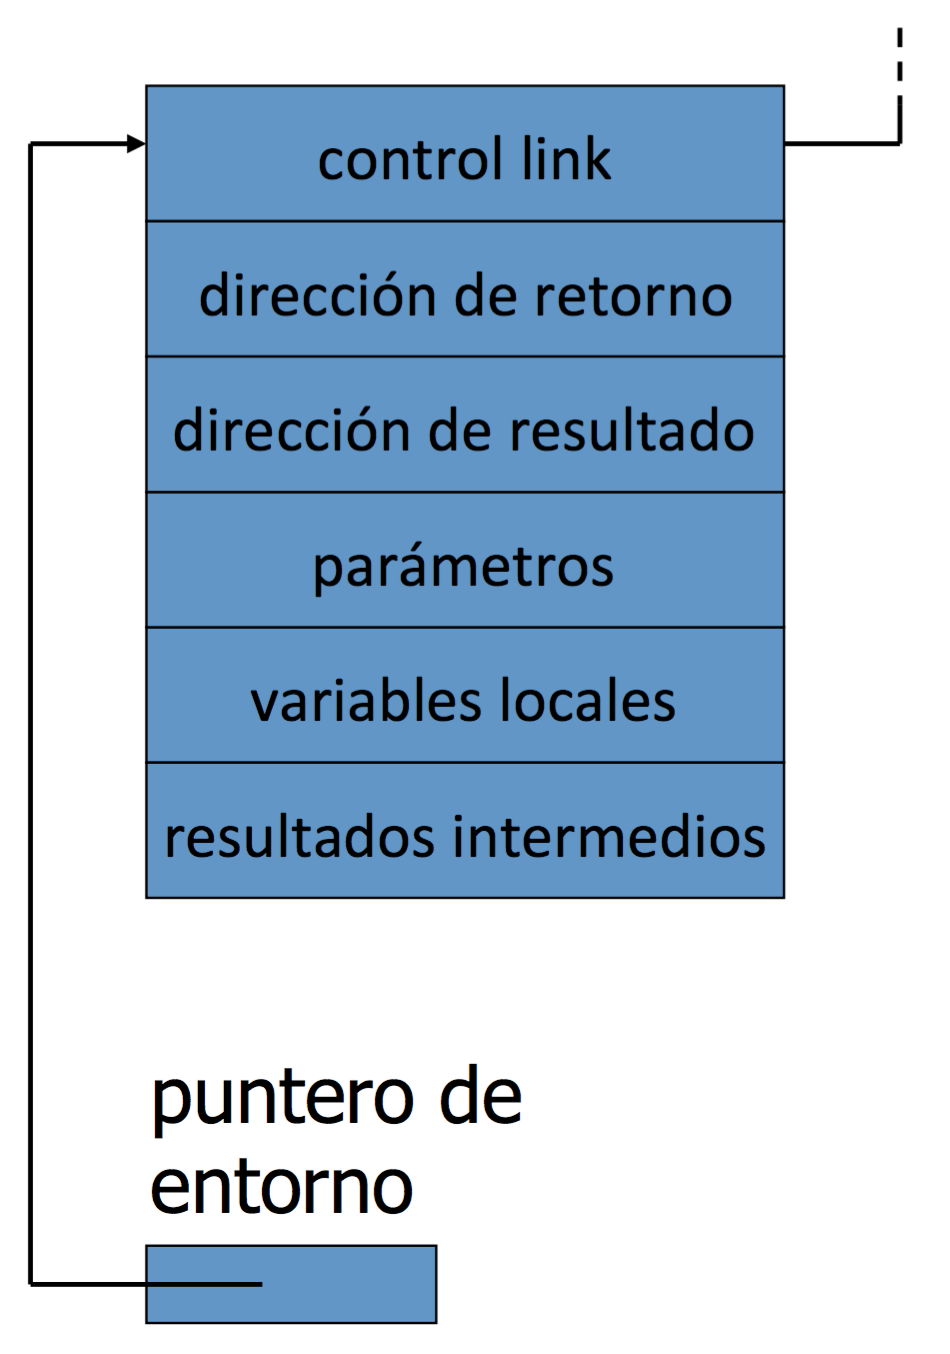
\includegraphics[width=6cm, height=6cm]{funcion.png}        
        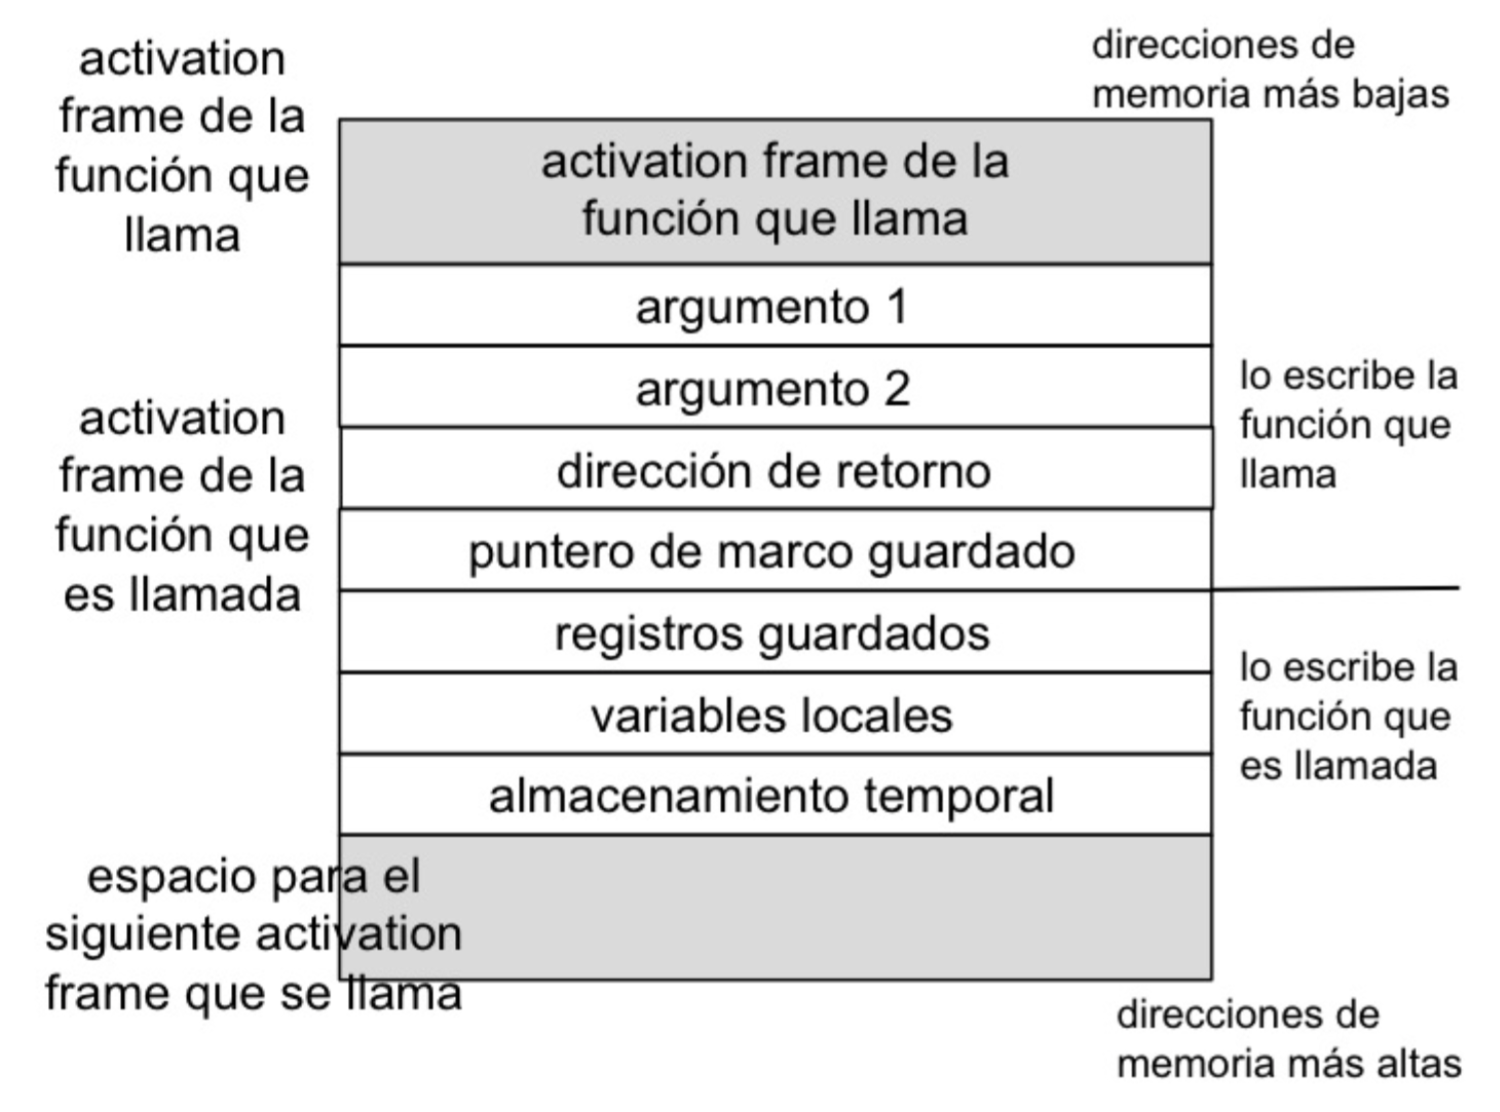
\includegraphics[width=8cm, height=6cm]{memoria.png}
\end{center}

\subsubsection{Ejemplo de activation record}

\begin{center}  
        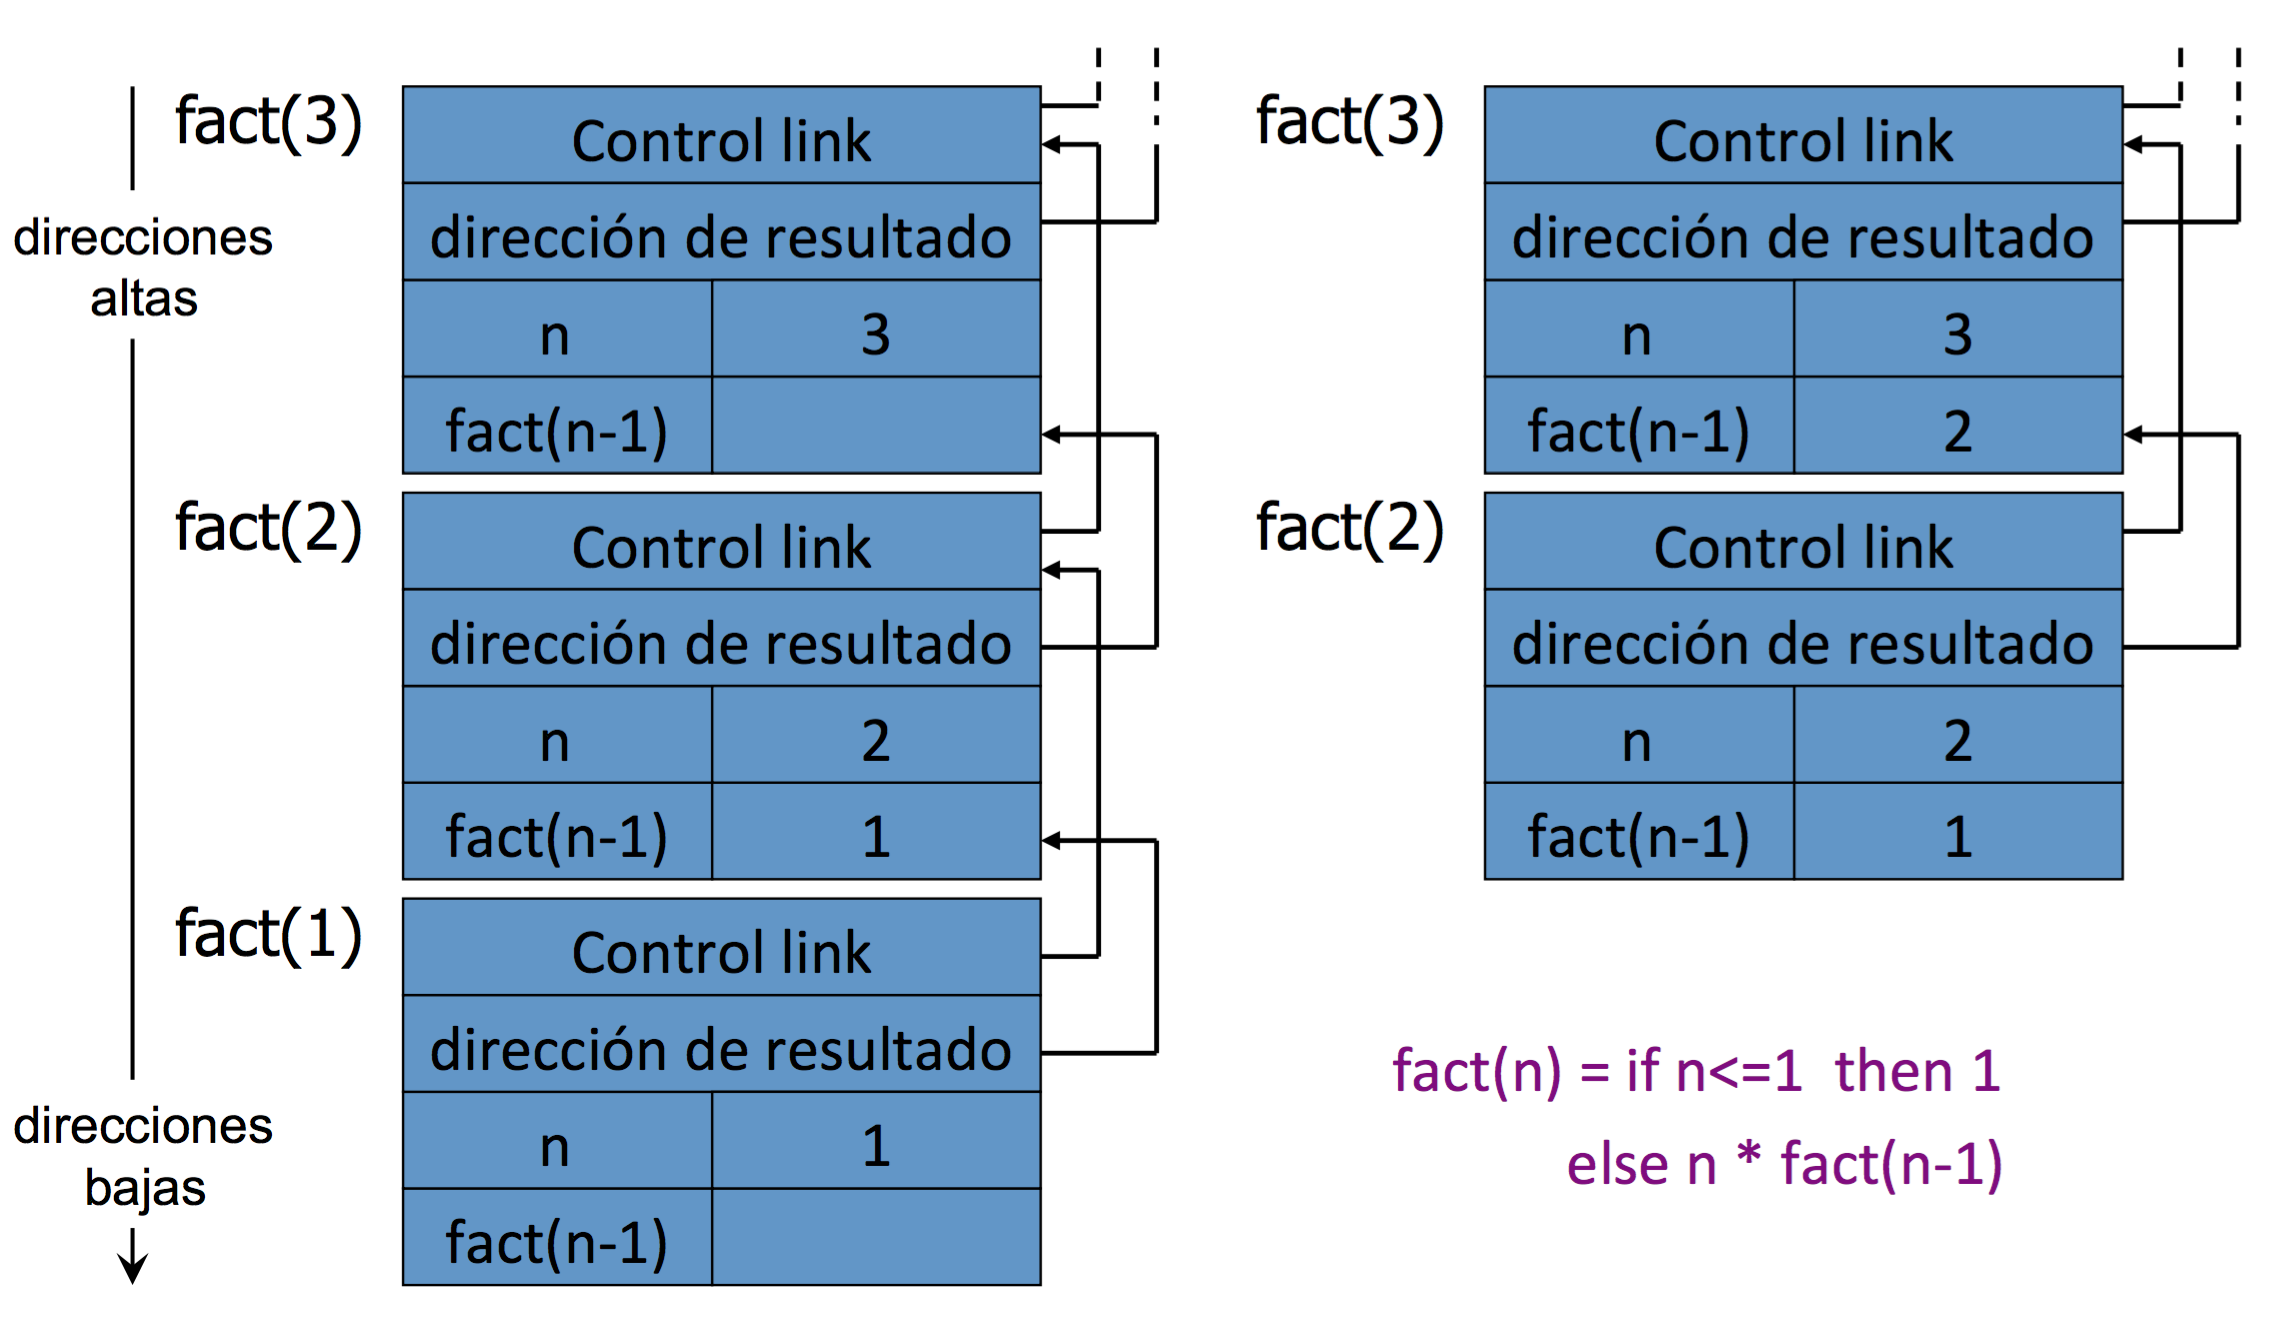
\includegraphics[width=10cm, height=8cm]{factorial.png}
\end{center}


\chapter{Control de la ejecución}

\section{Pasaje de parámetros}
\begin{enumerate}
    \item \underline{Pasaje por valor:} 
    \begin{itemize}
    \item La función que llama pasa el r-valor del argumento a la función. Es 
    necesario computar el valor del argumento en el momento de la llamada. 
    Reduce el \textit{aliasing} (dos identificadores para una sola ubicación en 
    memoria)
    \item  La función no puede cambiar el valor de la variable de la función 
    que llama
    \item Ejemplos: C, Java, Scheme. Se pueden pasar punteros si queremos 
    que se pueda modificar el valor de la variable de la función que llama
    \end{itemize}

    \item \underline{Pasaje por referencia:}
    \begin{itemize}
    \item La función que llama pasa el l-valor del argumento a la función. Se 
    asigna la dirección de memoria del argumento al parámetro. Aumenta el 
    \textit{aliasing}
    \item La función puede modificar la variable de la función que llama
    \item Ejemplos: C++, PHP
    \end{itemize}

    \item \underline{Pasaje por valor-resultado:}
    \begin{itemize}
    \item Intenta tener los beneficios de llamada por referencia (efectos 
    secundarios en los argumentos) sin los problemas de \textit{aliasing}
    \item Hace una copia en los argumentos al principio, copia las variables 
    locales a los argumentos actuales al final del procedimiento. Asi los 
    argumentos son modificados.
    \item Se comporta como llamada por referencia sin la presencia de   
    \textit{aliasing}
    \item Cuidado: el comportamiento depende del orden en que las 
    variables locales se copian.
    \item Ejemplos: BBC BASIC V
    \end{itemize}
    
    \item \underline{Pasaje por nombre:}
    \begin{itemize}
    \item En el cuerpo de la función se sustituye textualmente el argumento 
    para cada instancia de su parámetro. Se implementó para Algol 60 pero 
    sus sucesores no lo     incorporaron
    \item Es un ejemplo de ligado tardío. La evaluación del argumento se 
    posterga hasta que efectivamente se ejecuta en el cuerpo de la función.
    Asociado a evaluación perezosa en lenguajes funcionales (ej: Haskell)
    \end{itemize}
    
    \item \underline{Pasaje por necesidad:}
    \begin{itemize}
    \item Variación de call-by-name donde se guarda la evaluación del 
    parámetro después del primer uso
    \item Idéntico resultado a call-by-name (y más eficiente) si no hay 
    efectos secundarios
    \item El mismo concepto que lazy evaluation
    \end{itemize}

\end{enumerate}

\begin{center}  
        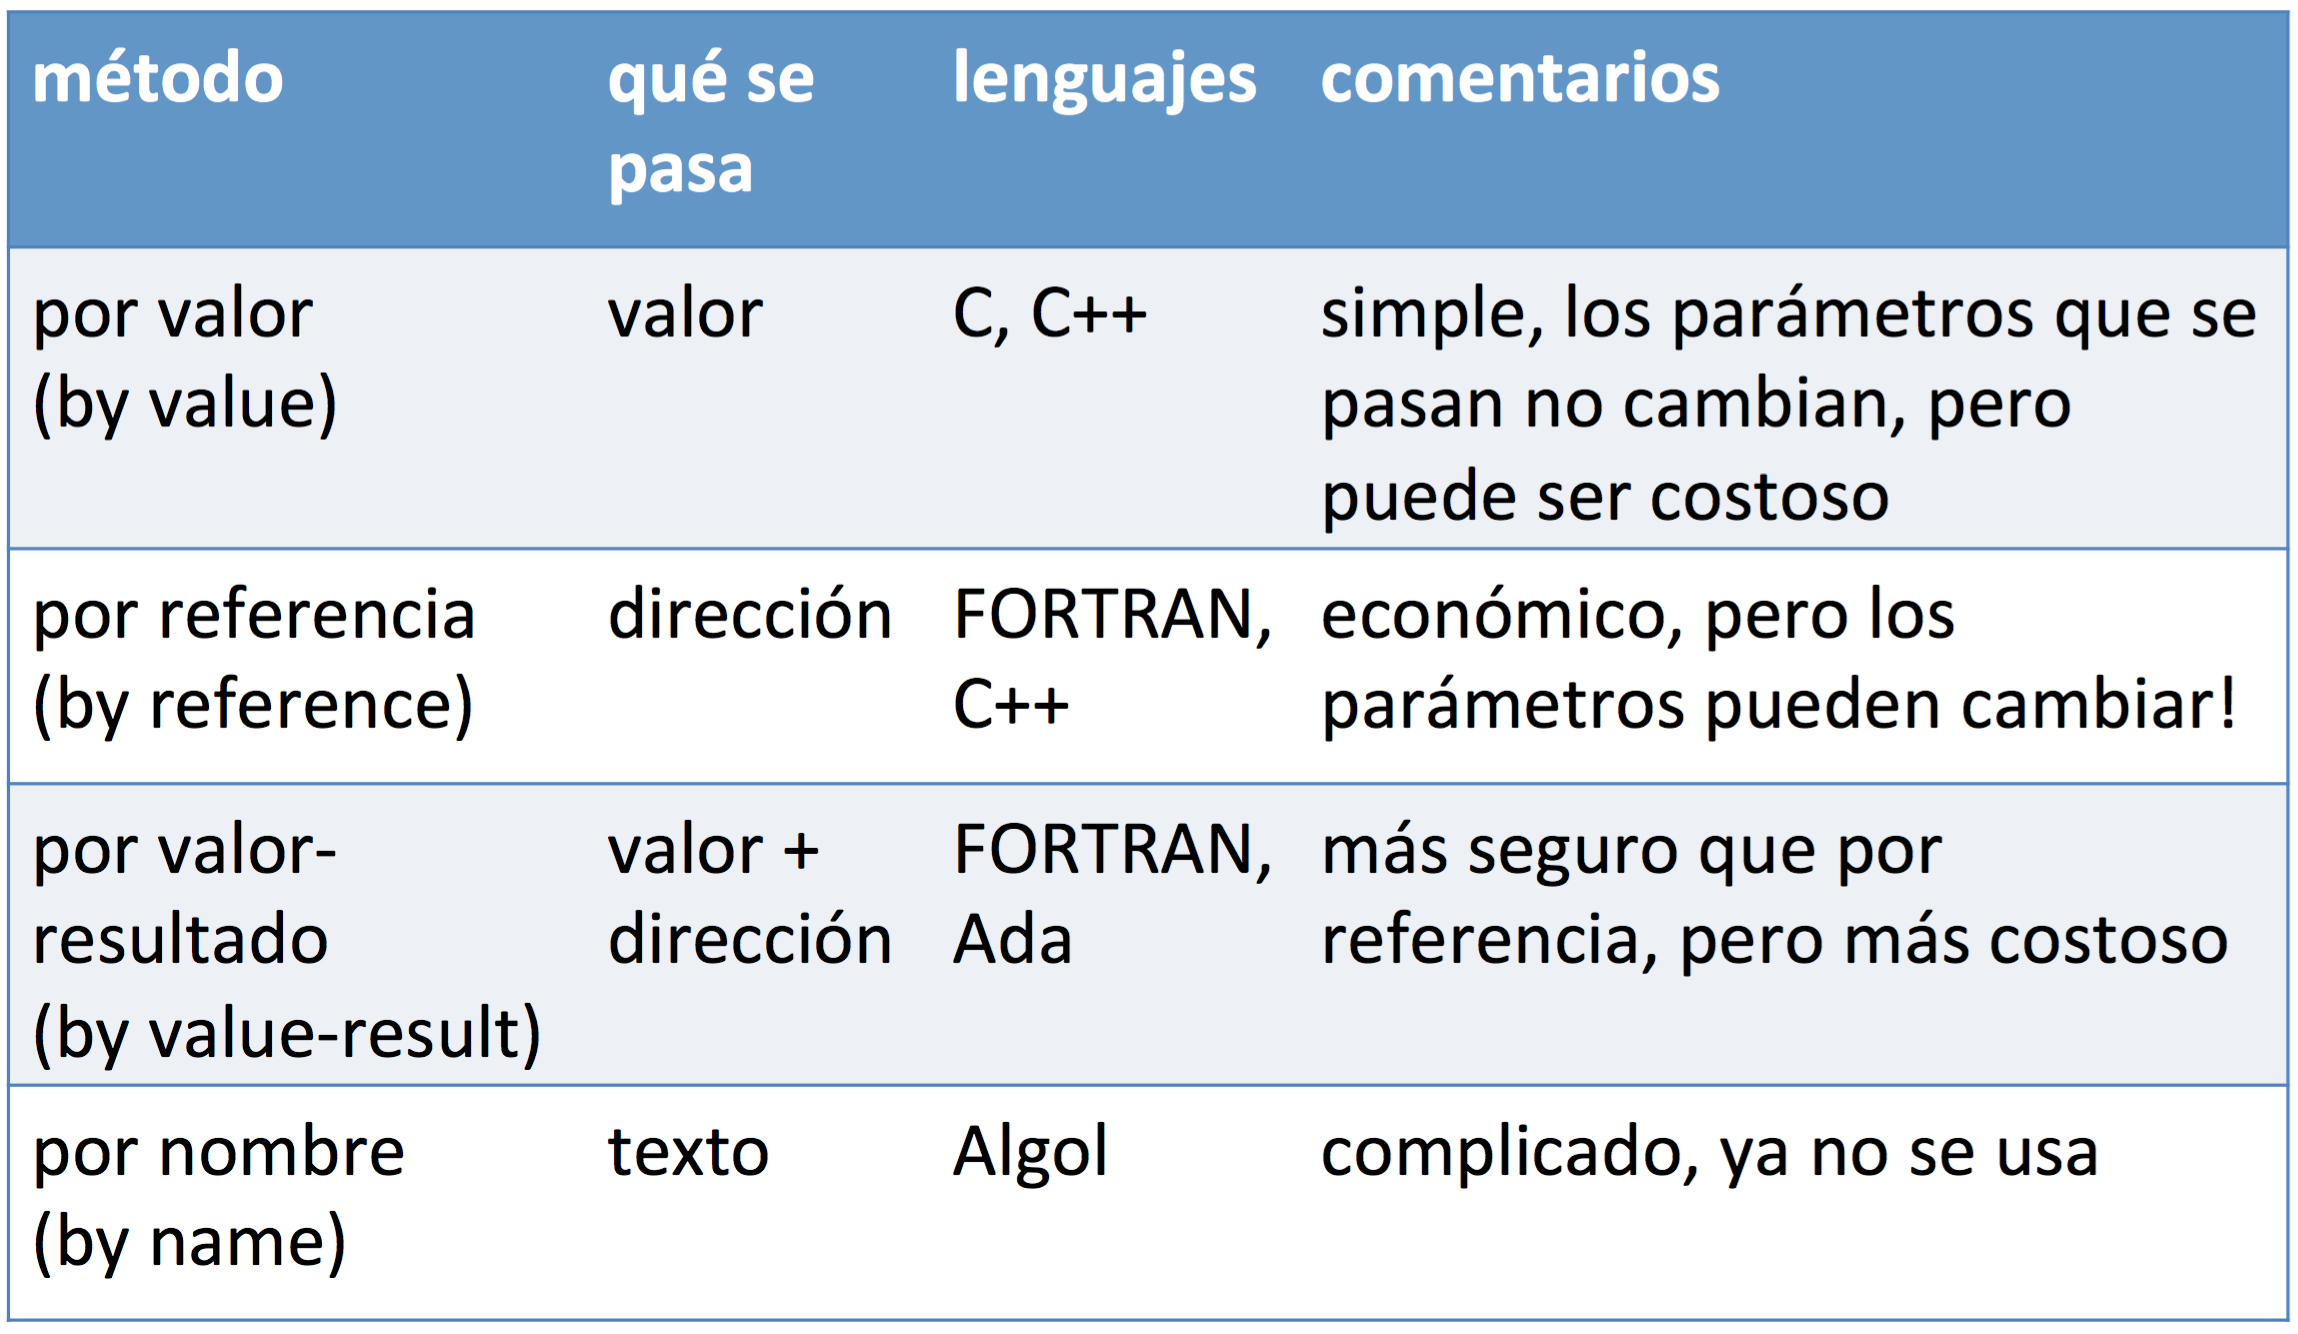
\includegraphics[width=12cm, height=8cm]{resumenpasajes.png}
\end{center}

\section{Alcance}
\par Si un identificador \verb|x| aparece en el cuerpo de una función, pero
\verb|x| no se declara dentro de la función, entonces el valor de
\verb|x| depende de alguna declaración fuera de la función. En esta
situación, la ubicación de \verb|x| está fuera del registro de
activación para la función y es una variable global a esa
función. Debido a que \verb|x| ha sido declarada en otro bloque, el
acceso a una \verb|x| libre o global consiste en encontrar el registro
de activación pertinente en la pila.

Hay dos políticas principales para buscar la declaración adecuada de
un identificador global:

\begin{description}
\item \underline{Alcance estatico:} un identificador global se refiere al identificador con ese nombre que se declara en el bloque contenedor más cercano del texto del programa.
\item \underline{Alcance dinamico:} un identificador global se refiere al identificador asociado con el registro de activación más reciente.
\end{description}

\par Aunque la mayoría de los lenguajes actuales de programación de
propósito general utilizan alcance estático para las declaraciones de
variables y funciones, el alcance dinámico es un concepto importante
que se utiliza en lenguajes de propósito específico y en
construcciones especializadas como las excepciones. Algunos lenguajes
con alcance dinámico son los dialectos antiguos de Lisp, los lenguajes
de marcado Tex/LaTex, las excepciones y las macros.

\begin{center}  
        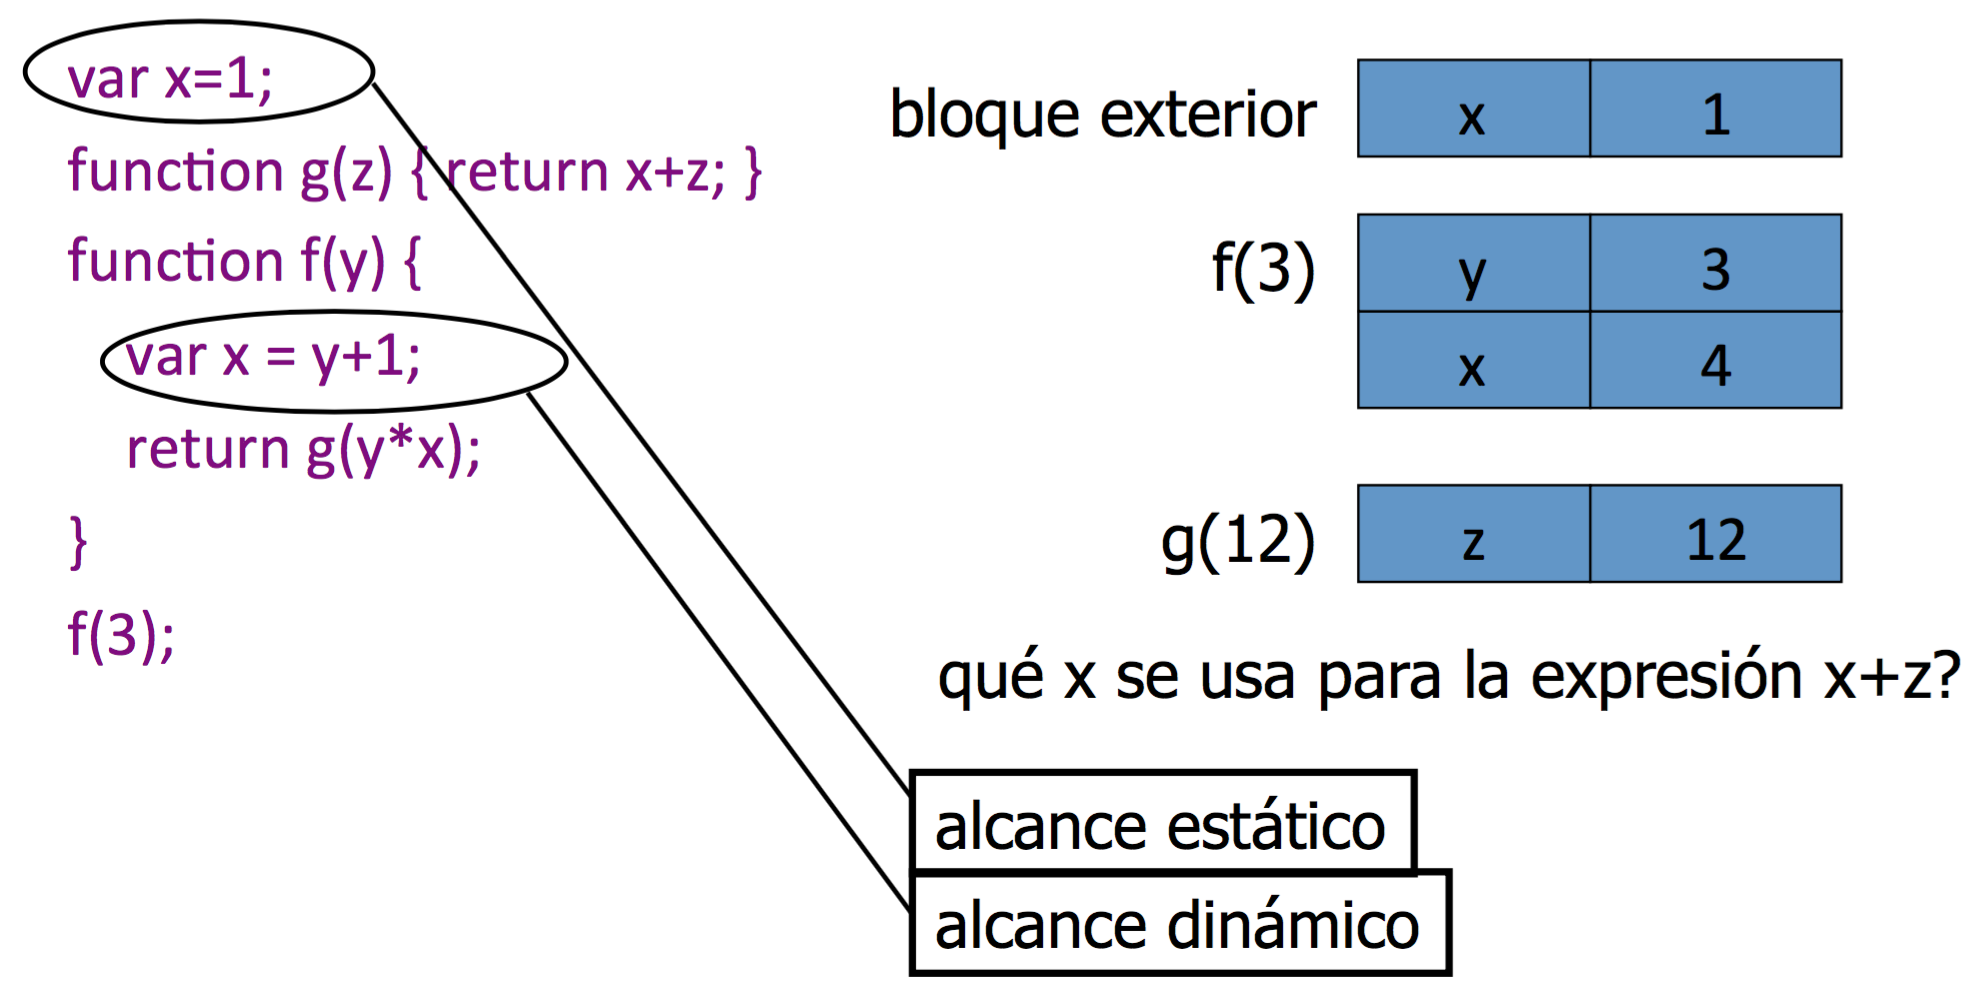
\includegraphics[width=12cm, height=6cm]{estaticodinamico.png}
\end{center}

\section{Alto orden}

\subsection{Funciones de primera clase}

Un lenguaje tiene función de primera clase si las funciones pueden ser
\begin{itemize}
\item declaradas dentro de cualquier alcance,
\item pasadas como argumentos a otras funciones y, 
\item devueltas como resultado de funciones.
\end{itemize}

En un lenguaje con funciones de primera clase y con alcance estático,
un valor de función se representa generalmente por una clausura,
un par formado por un puntero al código del cuerpo de una función y
otro puntero a un activation record.

Veamos un ejemplo de función en ML que requiere a otra función como argumento:

\begin{table}
 fun map (f, nil) = nil 
| map(f, x::xs) = f(x) :: map(f, xs)
\end{table}


La función \verb|map| toma una función \verb|f| y una lista \verb|xs|
como argumentos y aplica \verb|f| a cada elemento de \verb|xs| en
orden. El resultado de \verb|map(f, xs)| es la lista de resultados
\verb|f(x)| para elementos \verb|x| de la lista \verb|xs|. Esta función
es útil en muchos programas en los que se usan listas.

\subsection{Pasar funciones a otras funciones}

Vamos a ver que cuando una función \verb|f| se pasa a una función
\verb|g|, es posible que tengamos que pasar también la clausura de
\verb|f|, que contiene un puntero a su activation record. Cuando
\verb|f| se llama dentro del cuerpo de \verb|g|, el puntero de entorno
de la clausura se utiliza para determinar cuál es el access link que
tiene que guardarse en el activation record de la llamada a
\verb|f|. La necesidad de clausuras en este contexto se conoce como el
problema de \textit{downward funarg}, porque sucede cuando se pasan
funciones como argumentos hacia abajo en alcances anidados.

Vamos a ilustrar los principales aspectos de este problema con un 
programa de ejemplo con dos declaraciones de una variable \verb|x| y una función \verb|f| que se pasa a otra función \verb|g|:

val x = 4; 
fun f(y) = x*y; 
fun g(h) = let val x=7 in h(3) + x; 
g(f);

En este programa, el cuerpo de \verb|f| contiene una variable global
\verb|x| que se declara fuera del cuerpo de \verb|f|. Cuando \verb|f|
se llama dentro \verb|g|, el valor de \verb|x| se tiene que recuperar
desde el activation record asociado al bloque exterior. De lo
contrario el cuerpo de \verb|f| se evalúa con la variable \verb|x|
local declarada dentro de \verb|g|, lo cual es inconsistente con la
semántica de alcance estático.

Podemos ver el problema de la búsqueda de variables en la pila de
ejecución después de la llamada a \verb|f| desde la invocación de
\verb|g|.

\begin{center}

\end{center}

Esta ilustración simplificada muestra sólo los datos contenidos en
cada activation record. En esta ilustración, la expresión \verb|x * y|
del cuerpo de \verb|f| se muestra en la parte inferior, el activation
record asociado a la invocación de \verb|f| (a través del parámetro
formal \verb|h| de \verb|g|). Como muestra la ilustración, la variable
\verb|y| es local para la función y por lo tanto se puede encontrar en
el activation record actual. Sin embargo, la variable \verb|x| es
global, y se encuentra varios registros de activación por encima del
actual. Para encontrar las variables globales tenemos que seguir los
access links, por lo tanto el access link del activation record
inferior debe permitirnos alcanzar el activation record de la parte
superior de la ilustración.

Cuando las funciones se pasan a otras funciones, hay que guardar el
access link para el registro de la activación de cada función para que
podamos encontrar las variables globales de esa función según la
semántica del alcance estático. Y para poder cubrir este requisito
necesitamos extender alguna estructura de datos de tiempo de
ejecución. Esa estructura de datos serán las clausuras.

La solución estándar para mantener el alcance estático cuando las
funciones se pasan como argumentos a otras funciones o se devuelven
como resultados es utilizar una estructura de datos llamada
clausura. La clausura es un par formado por un puntero a la
parte de la memoria donde se guarda el código de la función y otro
puntero a un activation record. Debido a que cada activation record
contiene un access link señalando al activation record del bloque del
texto del programa más cercano que lo contiene, un puntero al alcance
en el que se declara una función también proporciona enlaces al
activation record del bloque que la contiene.

Cuando se pasa como parámetro una función a otra función, el valor
real que se pasa es un puntero a una clausura. A partir de una
clausura, una función se llama de la siguiente forma:

\begin{enumerate}
\item Asignar un activation record para la función que se llama, como
  es habitual.
\item Establecer el access link en el activation record utilizando el
  puntero del activation record de la clausura.
\end{enumerate}

Podemos ver cómo esto resuelve el problema de acceso a variables para
funciones que se pasan a otras funciones como argumentos. Para ello
vamos a diagramar el estado de la pila, con los diferentes activation
records, cuando se ejecuta el programa anterior, tal como se muestra
en la figura:

\begin{figure}

\end{figure}

Podemos entender la figura atravesando la
secuencia de pasos de ejecución que conducen a la configuración que se
muestra en la figura:

\begin{enumerate}
\item Declaración de \verb|x|: se apila un activation record para el
  bloque en el que se declara \verb|x|. El activation record contiene
  un valor para \verb|x| y un control link que no se muestra.
\item Declaración de \verb|f|: se apila un activation record para el
  bloque en ue se declara \verb|f|. Este activation record contiene un
  puntero a la representación en tiempo de ejecución de \verb|f|, que
  es una clausura con dos punteros. El primer puntero apunta al
  activation record para el alcance estático de \verb|f|, que es el
  activation record para la declaración de \verb|f|. El segundo
  puntero apunta al código de verb|f|, que fue producido durante la
  compilación y se coloca en alguna ubicación de memoria que conoce el
  compilador.
\item Declaración de \verb|g|: Al igual que con la declaración de
  \verb|f|, se apila un activation record para el bloque en el que se
  declaró \verb|g|. Este activation record contiene un puntero a la
  representación en tiempo de ejecución de \verb|g|, que es una
  clausura.
\item Llamada a \verb|g(f)|: La llamada hace que se apile un
  activation record para la función \verb|g|. El tamaño y estructura
  de este record los determina el código para \verb|g|. El access link
  se establece hacia el activation record para el alcance donde se
  declara \verb|g|; el access link apunta al mismo activation record
  que el activation record que hay en la clausura de \verb|g|. El
  activation record tiene espacio para el parámetro \verb|h| y la
  variable local \verb|x|. Debido a que el parámetro real es la
  clausura de \verb|f|, el valor del parámetro \verb|h| es un puntero
  a la clausura de \verb|f|. La variable local \verb|x| tiene un valor
  de 7, que viene dado por el código fuente.
\item Llamada a \verb|h(3)|: El mecanismo para la ejecución de esta
  llamada es el punto principal de este ejemplo. Debido a que \verb|h|
  es un parámetro formal de \verb|g|, el código de \verb|g| se compila
  sin saber dónde se declara la función \verb|h|. Como resultado, el
  compilador no puede establecer el access link para el activation
  record para la llamada \verb|h(3)|. Sin embargo, la clausura provee
  esa información: el access link para este activation record se
  establece mediante el puntero de activation record de la clausura de
  \verb|h|. Debido a que el parámetro real es \verb|f|, el acces link
  apunta al activation record para el alcance en el que se declaró
  \verb|f|. Cuando se ejecuta el código de \verb|f|, el access link se
  utiliza para encontrar \verb|x|. En concreto, el código seguirá el
  access link hasta el segundo activation record de la ilustración,
  seguirá un access link adicional porque el compilador sabía, cuando
  generó el código para \verb|f|, que la declaración de \verb|x| se
  encuentra un alcance por encima de la declaración de \verb|f|, y
  encontrará el valor 4 para la variable global \verb|x| en el cuerpo
  de \verb|f|.
\end{enumerate}

Como se describe en el paso 5, la clausura de \verb|f| hace posible
que el código que se ejecuta encuentre el activation record que
contiene la declaración global de \verb|x|.

Cuando podemos pasar funciones como argumentos, los access links
dentro de la pila forman un árbol. La estructura no es lineal, porque
el activation record correspondiente a la llamada a la función
\verb|h(3)| tiene que saltar el activation record para \verb|g(f)|
para encontrar el \verb|x| adecuado. Sin embargo, todos los access
links apuntan hacia arriba. Por lo tanto, sigue siendo posible asignar
y desasignar activation records mediante el uso de la disciplina de
pila (último apilado, primero desapilado).


\section{Recursión a la cola}
\par Una optimización que realizan los compiladores es la llamada eliminación de la recursion a la cola. Para las funciones recursivas a la cola, que describimos a continuación, se puede reutilizar un activation record para una llamada recursiva a la
función. Esto reduce la cantidad de espacio de la pila que usa una
función recursiva, y evita llegar a problemas por límites de hardware
como el llamado {\it stack overflow}, en el que la ejecución de un
programa requiere más espacio del que hay disponible en la pila.

Una llamada a \verb|f| en el cuerpo de \verb|g| es una
llamada de la cola si \verb|g| devuelve el resultado de la llamada
\verb|f| sin ningún cálculo adicional. Una función \verb|f| es recursiva de cola si todas las llamadas recursivas en el cuerpo de \verb|f| son llamadas a la cola a \verb|f|. 

Veamos como ejemplo la función recursiva a la cola que calcula el factorial:

\begin{tabbing}
fun factcola(n,a) = if n <= 1 then a else factcola(n-1, n * a);
\end{tabbing}

La ventaja de la recursión de cola es que podemos utilizar el mismo activation record para todas las llamadas recursivas.

    \begin{center}  
        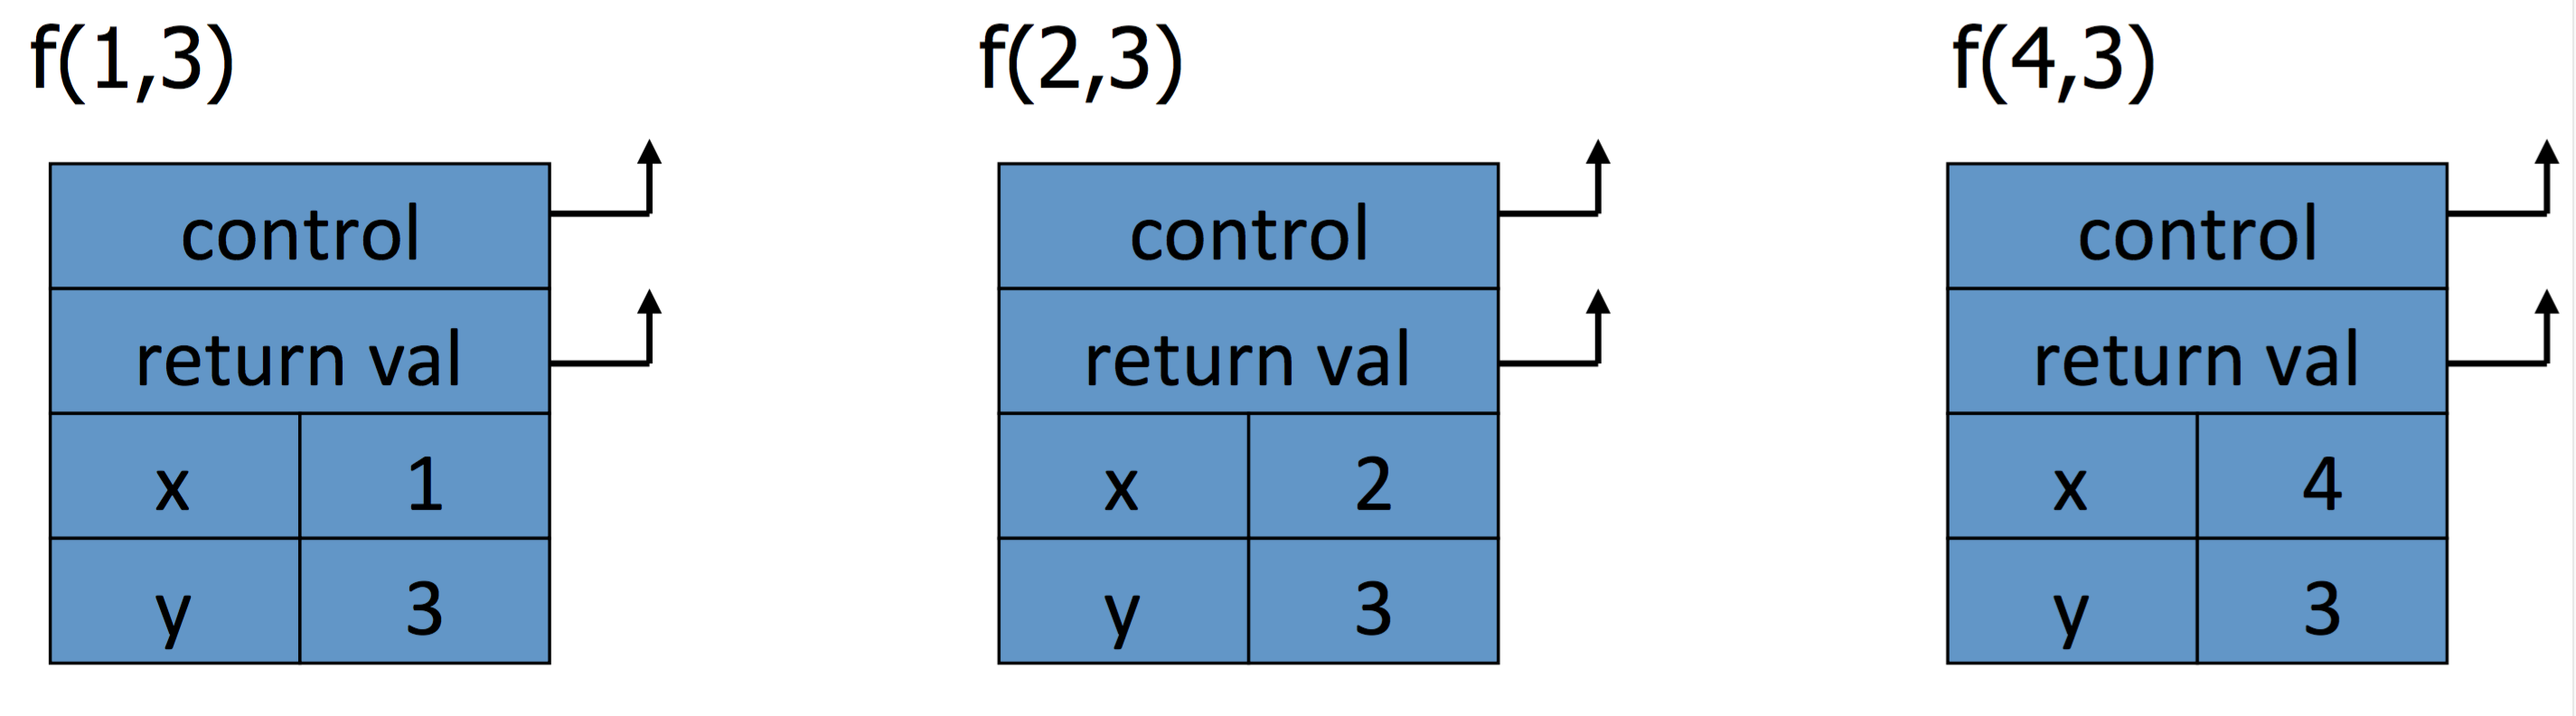
\includegraphics[width=12cm, height=6cm]{factorial2.png}
    \end{center}

\section{Excepciones}

Las excepción proporcionan una forma estructurada de salto que se
puede utilizar para salir de una construcción tal como un bloque o
llamada a función. El nombre de excepción sugiere que las excepciones
deben ser utilizados en circunstancias excepcionales. Sin embargo, es
muy habitual usarlas de formas muy poco excepcionales, como por
ejemplo:

\begin{itemize}
\item salir de un bloque o llamada de función
\item pasar datos como parte de un salto
\item volver a un punto del programa fijado para continuar la computación
\end{itemize}

Además de saltar de un punto a otro del programa, también se asocia
con las excepciones parte del manejo de memoria. Más en concreto, se
pueden desapilar activation records que ya resulten innecesarios como
resultado del salto.

Todo mecanismo de excepción incluye dos construcciones lingüísticas:

\begin{itemize}
\item {levantar}, {\it rise} o {\it throw}, una construcción para
  ejecutar una excepción, que corta parte del cómputo actual y provoca
  un salto (transferencia de control),
\item un controlador, {\it handle} o {\it catch}, un mecanismo
  de control, que permite ciertas declaraciones, expresiones o
  llamadas a función provistos de código para responder a las
  excepciones que se lanzan durante la ejecución.
\end{itemize}

Hay varias razones por las que las excepciones se han convertido en
construcciones muy aceptadas en la mayor parte de lenguajes. Muchos
lenguajes no tienen ningún otro mecanismo limpio para saltar fuera de
una llamada de función, por ejemplo, abortando la llamada. En lugar de
utilizar instrucciones del tipo \verb|go to|, que permiten crear
código totalmente desestructurado (\textit{spaghetti}), muchos
programadores prefieren usar excepciones, que se pueden utilizar para
saltar sólo hacia la parte del programa que ya se ha cargado en la
pila, no hacia alguna parte del programa que no se ha ejecutado
todavía.

Las excepciones también permiten a un programador pasar datos como
parte del salto, lo cual resulta muy útil si el programa trata de
recuperarse de algún tipo de condición de error. Las excepciones
proporcionan un método dinámico y útil de determinar hasta donde llega
un salto. Si se declara más de un mecanismo de control, se establece
cuál es el controlador adecuado en cada caso siguiendo una semántica
de alcance dinámico, lo cual no sería fácil de lograr con otras formas
de saltos de control.


\subsubsection{Excepciones en ML}

Declaración: exception <name> of <type>. Dá el nombre de la excepción y el tipo de dato que se pasa cuando se levanta
Levantado: raise <name> <parameters>
Manejador: <exp1> handle <pattern> =>
<exp2>. Evaluar la primera expresión, si la excepción levantada se corresponde con el patrón (pattern-matching), se evalúa la segunda expresión.


\subsubsection{Tipado de las excepciones}

tipado de raise exn
–  definición de tipado: la expresión e tiene el tipo t si la terminación normal de e produce un valor de tipo t 
–  levantar una excepción no es una terminación normal 1 + raise X 
•  tipado de handle exception => value
–  convierte una excepción a terminación normal
–  implementa acuerdo de tipos • 1+((raiseX)handleX=>e)  
el tipo de e tiene que ser int •  1 + (e1 handle X => e2)
el tipo de e1, e2 tiene que ser int

\chapter{Orientación a objetos}

\section{Modularidad: conceptos básicos}
\par Definamos los conceptos básicos acompañandolos con un ejemplo
\begin{itemize}
    \item componente: unidad de programa con sentido: función, estructura de 
    datos, módulo.
    
    Función que calcula la raíz cuadrad.
    \item interfaz: tipos y operaciones definidos dentro de un componente que son 
    visibles fuera del componente.
    
      float sqroot (float x) 
    \item especificación: comportamiento esperado de un componente, expresado 
    como una propiedad observable a través de la interfaz.
    
    si x$>$1, entonces sqrt(x)*sqrt(x) x 
    \item implementación: estructuras de datos y funciones dentro del componente

   float sqroot (float x){ 
       float y = x/2; float step=x/4; int i; 
       for (i=0; i<20; i++){if ((y*y)<x) y=y+step; else y=y-step;
      step = step/2;} 
return y;  }
\end{itemize}


\section{Tipos abstractos de datos (TADs)}
Este era el desarrollo de lenguaje de los 1970s, consistía de dos ideas:
\begin{itemize}
    \item Idea 1: separar la interfaz de la implementación
    \textbf{Ejemplo:} los conjuntos tienen las operaciones: empty, insert, union, is member?, etc
    los conjuntos se implementan como lista enlazada, etc.
    \item Idea 2: usar comprobación de tipos para forzar la separación. El programa 
    cliente sólo tiene acceso a las operaciones de la interfaz, la implementación está 
    encapsulada en el constructo TAD.
\end{itemize}

\section{Módulos}

\par Los módulos son una construcción general para ocultar información, son 
llamados módulos en Modula, paquetes en Ada, estructuras en ML. Con módulos se 
puede definir un TAD con tipo privado y operaciones públicas, los módulos son más generales, pueden incluir varios tipos y operaciones relacionados; algunos lenguajes separan interfaz e implementación, de forma que una interfaz puede tener múltiples implementaciones.

\subsubsection{Abstracciones genéricas }
\par Parameterizar los módulos por tipos. Implementaciones generales, que se 
pueden instanciar de muchas formas: la misma implementación para múltiples tipos. 
Paquetes genéricos en Ada, templates en C ++ (especialmente las de la STL – 
Standard Template Library), functores en ML functors

\subsection{Templates de C++}
\par Un template es un mecanismo de parametrización de tipos, 
template<class T>, indica el parámetro de tipo T. C++ tiene templates de clase y de 
función, se instancian en tiempo de ligado, se crea una copia del template generado 
para cada tipo ya que el tamaño de las variables locales en el activation record está 
ligado a las operaciones del tipo instanciado. Por ejemplo: la función swap definida a 
continuación.

\par Ejemplo de template:
 
template <typename T>  
void swap(T x, T y){ 
T tmp = x;  x=y;  y=tmp; 
} 


\subsubsection{Diferencia entre ML y C++}
    \begin{itemize}
        \item ML: Swap se compila a una función, y el typechecker determina cómo se puede usar. La x local es un puntero a un valor en el heap, con tamaño constante.
        \item C++: Swap se compila a formato linkeable, y el linker duplica el código para cada tipo con el que se usa. La x local es un puntero a un valor en el stack, su tamaño depende del tipo.

    \end{itemize} 

\subsection{C++ Standard Template Library}

muchas abstracciones genéricas
operaciones tipos abstractos polimórficos –  ejemplo de programación genérica
eficiente en tiempo de ejecución (pero no siempre en espacio)
escrito en C++
usa el mecanismo de templates y sobrecarga –  no usa objetos – no hay funciones 
virtuales

\section{Programación orientada a objetos}
\par Un objeto consiste de datos ocultos, como variables de la instancia y 
posiblemente funciones ocultas, y operaciones públicas como métodos y puede 
tener variables públicas en algunos mensajes. Un programa orientado a objetos 
envía mensajes a los objetos. Algunos conceptos importantes de lenguaje son:
\begin{itemize}
\item Lookup dinámico: en programación convencional, el significado de una 
operación con los mismos operandos es siempre el mismo.
  operación(operandos) 
En programación orientada a objetos, el código depende del objeto y el mensaje
object message (arguments) 
\par Esta es la diferencia fundamental entre TADs y objetos.

\subsubsection{Sobrecarga vs. lookup dinámico}
•  en programación convencional add (x, y)  la función add tiene significado fijo
•  para sumar dos números x  add (y) 
tenemos un add distinto si x es entero, complejo,
etc.
•  semejante a la sobrecarga, con una diferencia crítica: la sobrecarga se resuelve en 
tiempo de compilación, mientras que el lookup dinámico se resuelve en tiempo de 
ejecución
    \item Encapsulación: •  el constructor de un concepto tiene una vista detallada
•  el usuario de un concepto tiene una vista abstracta
•  la encapsulación separa estas dos vistas, de forma que el código de cliente opera con un conjunto fijo de oparciones que provee el implementador de la abstracción
    
    \item Subtipado y herencia: la interfaz es la vista externa de un objeto
•  el subtipado es una relación entre interfaces
•  la implementación es la representación interna de un objeto
•  la herencia es una relación entre implementaciones, de forma que nuevos objetos se pueden definir reusando implementaciones de otros objetos


interfaces de objeto •  interfaz
– los mensajes que entiende un objeto •  ej: Punto 
– x-coord : devuelve la coordenada x de un punto
– y-coord : devuelve la coordenada y de un punto
– move : método para cambiar de ubicación •  la interfaz de un objeto es su tipo


subtipado
•  si la interfaz A contiene todos los elementos de la interfaz B, entonces los 
objetos de tipo A también se pueden usar como objetos de tipo B
Punto
x-coord y-coord move
Puntocoloreado
x-coord y-coord
color
move changecolor
la interfaz de Puntocoloreado conHene la de Punto, por lo tanto Puntocoloreado es un subyipo de Punto 



Subtipado: Coloredpoint se puede usar en lugar de Point: propiedad que usa el cliente
•  Herencia: Coloredpoint se puede implementar reusando la impelementación de Point: propiedad que usa el implementador

estructura de un programa orientado a objetos
•  agrupar datos y funciones •  clase
– define el comportamiento de todos los objetos que son instancias de la clase
•  subtipado
– organiza datos semejantes en clases
relacionadas •  herencia
– evita reimplementar funciones ya definidas


\end{itemize}








\end{document}
